% !TeX program = lualatex
\documentclass[a0paper,landscape]{baposter}

\usepackage[EU1]{fontenc}
\usepackage{fontspec}
\defaultfontfeatures{Ligatures=TeX}
\setromanfont{TeX Gyre Schola}
\setsansfont{TeX Gyre Adventor}
\setmonofont{TeX Gyre Cursor}
\usepackage{microtype}

\usepackage{setspace}

\usepackage{fancyvrb}

% TODO change this
\usepackage{lyluatex}

\definecolor{lilyLightHeader1}{RGB}{212,242,201}
\definecolor{lilyLightHeader2}{RGB}{140,210,118}
\definecolor{lilyDarkHeader}{RGB}{91,127,100}


\begin{document}
\begin{poster}{%
	columns=5,
	background=none,
  % Show grid to help with alignment
	grid=false,
% Column spacing
	colspacing=1em,
% Color style
	bgColorOne=white,
	bgColorTwo=lilyLightHeader1,
	borderColor=lilyDarkHeader,
	headerColorOne=white,
	headerColorTwo=lilyLightHeader1,
	headerFontColor=lilyDarkHeader,
	boxColorOne=lilyLightHeader1,
	boxColorTwo=lilyLightHeader2,
% Format of textbox
	textborder=faded,
% Format of text header
	eyecatcher=true,
	headerborder=closed,
	headerheight=0.1\textheight,
    % textfont=\sc, % An example of changing the text font
	headershape=smallrounded,
	headershade=shadetb,
    % headerfont=\Large\bf\textsc, %Sans Serif
    % textfont={\setlength{\parindent}{1.5em}},
	boxshade=plain,
%   background=shade-tb,
	background=plain,
	linewidth=2pt
	}
% eyecatcher
  {
  	
\includegraphics[width=0.11\linewidth]{double-lily-modified3.png}
  }
% title
  {GNU LilyPond}
% author
  {http://lilypond.org/}
% university
  {
\includegraphics[width=.11\textwidth]{double-lily-modified3.png}}
%%%%%%%%%%%%%%%%%%%%%%%%%%%%%%%%%%%%%%%%%%%%%%%%%%%%%%%%%%%%%%%%%%%%%%%%%%%%%%%
%%% Content

  \headerbox{Text Input}{name=text,column=0,span=1,boxpadding=12pt}{
LilyPond is a text based system; the input is a text file describing the music, as opposed to a
“What You See Is What You Get” graphical application where you might drag notes from a toolbar onto
your on-screen score. In this way, LilyPond shares many similarities with programming and script
languages: The text input is interpreted (or “compiled”) by LilyPond  which produces typeset music.
\\

This might seem old-fashioned, or even clumsy, but it is in fact surprisingly easy to start using
LilyPond  and the results you will get are both predictable and beautiful. People accustomed to
graphical user interfaces will need to learn a new way of working, but the results are definitely
worth it!
  }

\headerbox{Basic Note Entry}{name=note-entry,column=1,span=1,boxpadding=12pt}{
	Note entry is as easy as typing the note name and the duration.

	\VerbatimInput{lily/note-entry.ly}

	\lilypondfile{lily/note-entry.ly}

	Append \texttt{is} for sharp and \texttt{es} for flat tones. Duration is specified with
	\texttt{4} for fourths, \texttt{8} for eigths, and so on. Create dotted notes by appending
	dots to the duration digit. Pitch is specified using a variant of the Helmholtz pitch
	notation.

}

\headerbox{Figured Bass Entry}{name=figures,column=1,span=1,boxpadding=12pt,row=.48}{
	It is easy to add a figured bass.\vspace{1em}

	\texttt{<7\textbackslash+ 4 2>8 <8> <7!>}\vspace{1em}

    \lilypondfile{lily/figured-bass.ly}

	A group of bass figures is delimited by `<' and `>', with the duration immediately appended.
	Accidentals are entered by appending `+' for sharps, `-' for flats, or `!' for naturals,
	immediately after each number.
}

\headerbox{Chord Entry}{name=chords,column=0,span=1,boxpadding=12pt,below=text}{
	It is easy to write out chords.\vspace{1em}

	\texttt{\textbackslash chordmode \\ \{ d4:m7 g c2:maj7 \}}
	\vspace{1em}

	First, specify the root note, then add the duration. Any modifiers can be added by
	appending `:', followed by a list of the modifiers.

	\lilypondfile{lily/chords.ly}
}

\headerbox{Variables}{name=variables,column=2,span=2,boxpadding=12pt}{
	\begin{minipage}{.7\textwidth}
	A powerful feature of LilyPond, is variables. Write once, then choose how you want to
	display the music! For example, here's a short polyphonic sequence:
	\vspace{.5em}

	\texttt{myMusic = \{ <c' e' g'> <d' f' a'> <e' g' b'> <f' a' c''> \}}
	\vspace{.3em}

	Then, we'll display this as chord names, as notes, as guitar tablature, and as a fretboard
	diagram, simply by referencing the variable:
	%\vspace{.1em}
	
	\texttt{\noindent
	\textbackslash new ChordNames \textbackslash myMusic\\
	\textbackslash new FretBoards \textbackslash myMusic\\
	\textbackslash new Staff \textbackslash myMusic\\
	\textbackslash new Tablature \textbackslash myMusic\\
	}
	\end{minipage}\hfill
	\begin{minipage}{.18\textwidth}
	\lilypondfile{lily/variables.ly}
	\end{minipage}
}

  \headerbox{Classical Music}{name=classical,column=2,span=1,row=.34}{
  	Excerpt from the Markus Passion by Johann Sebastian Bach (BWV 247)

	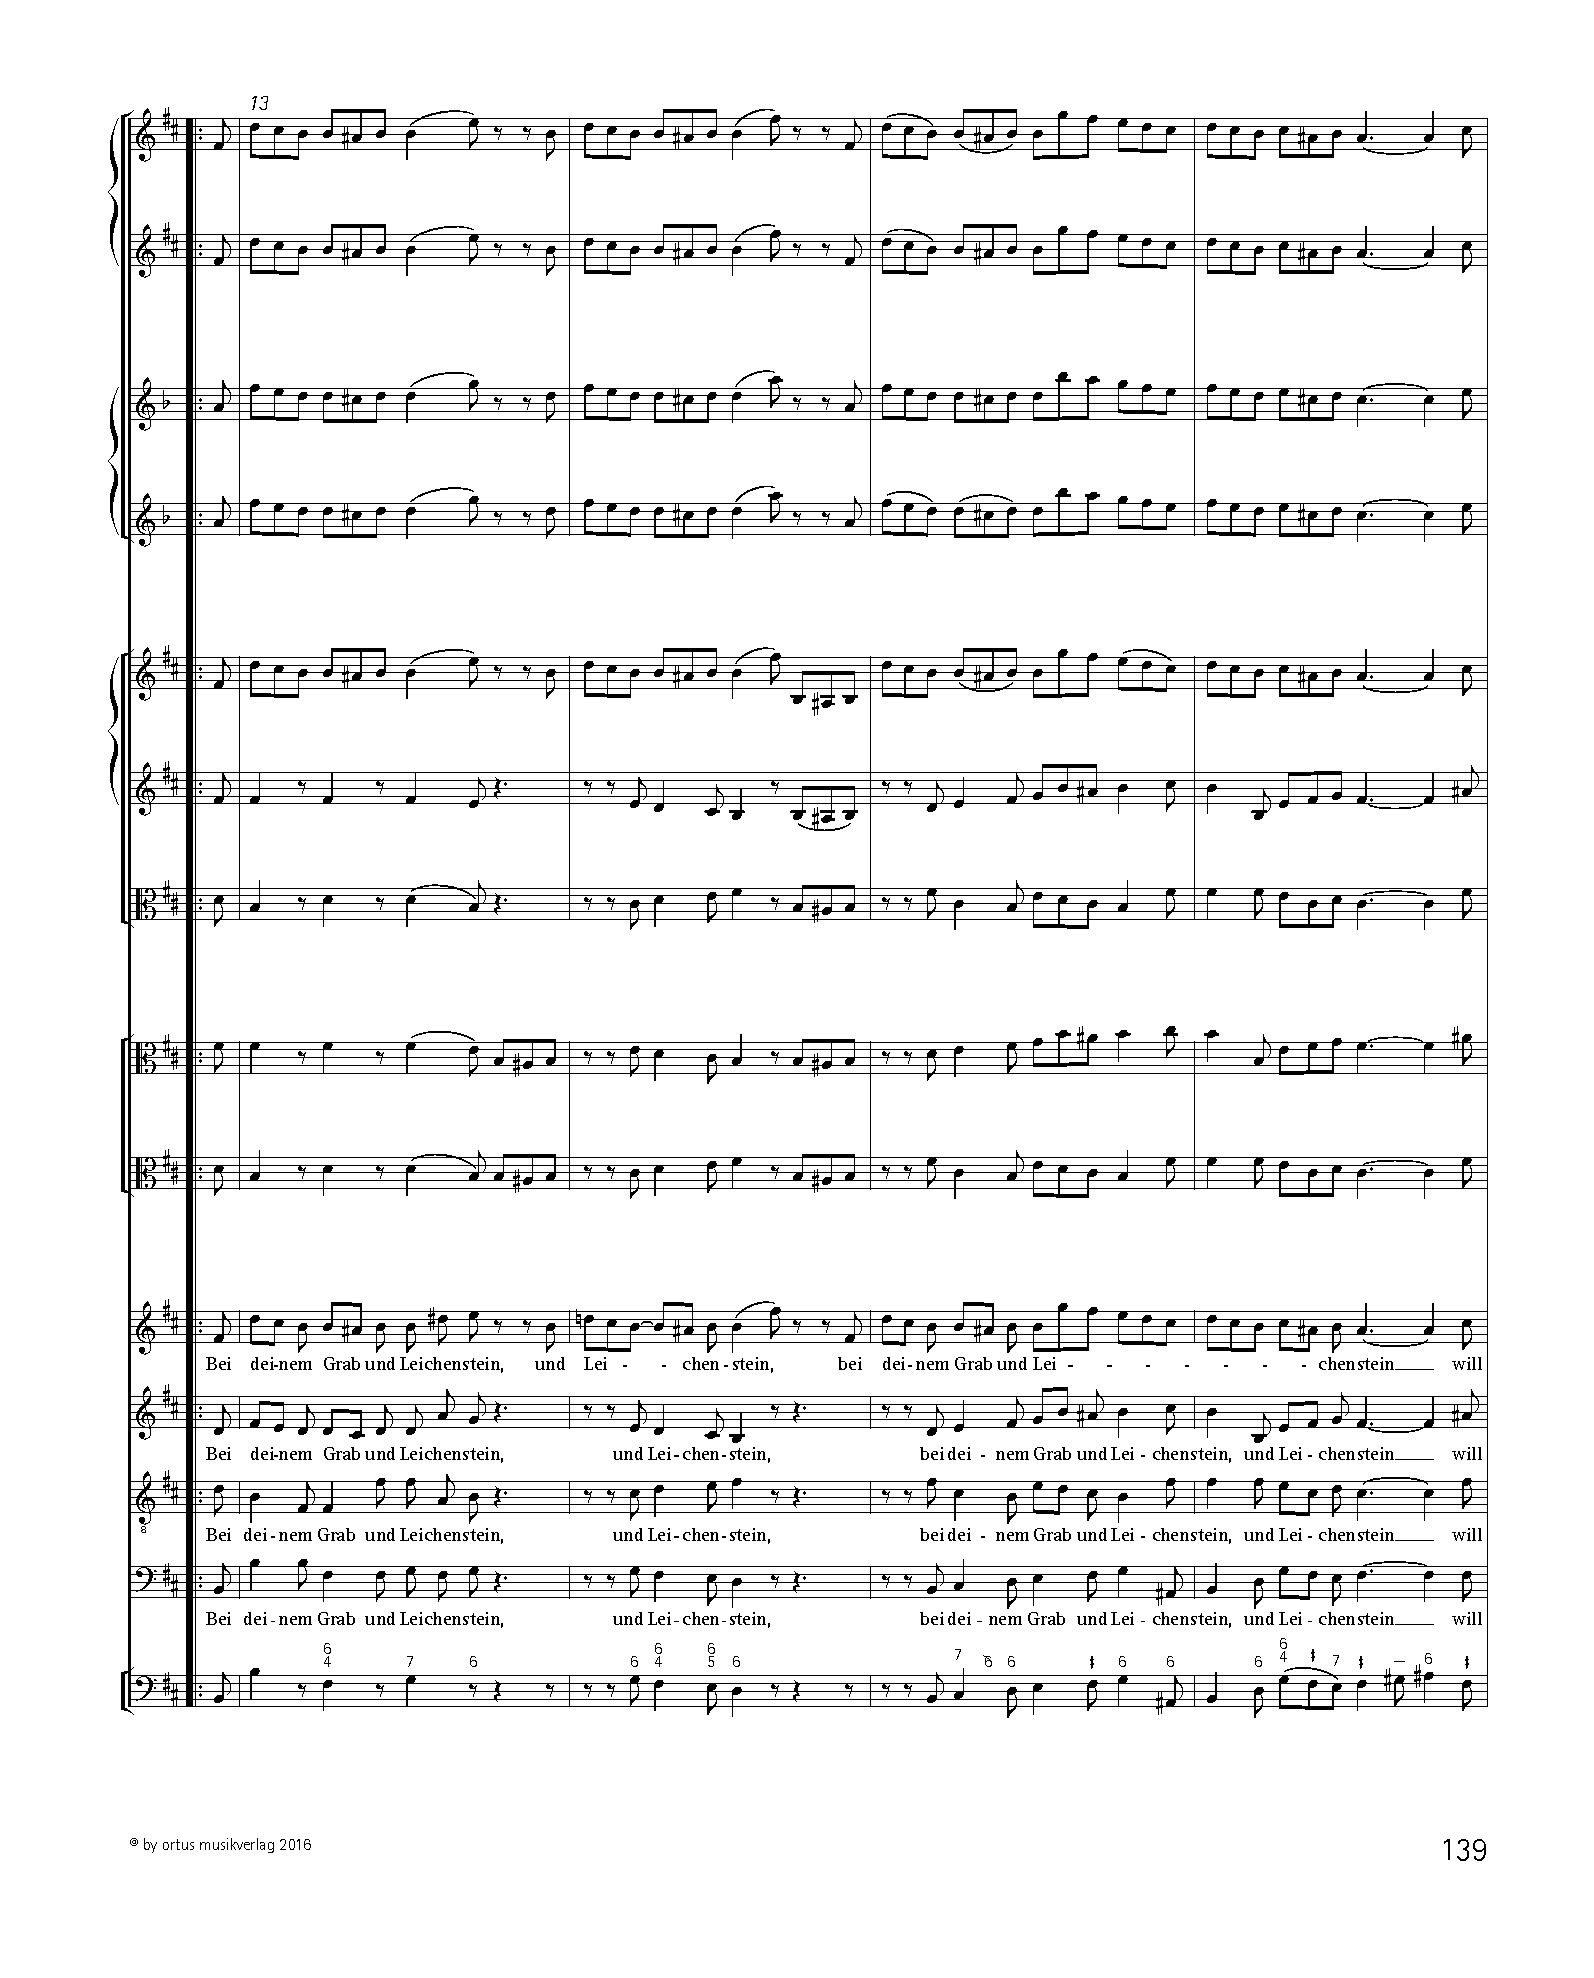
\includegraphics[width=\textwidth]{bwv247-partitur1.pdf}

	{\scriptsize © 2016 Ortus Musik Verlag, Berlin $\bullet$
	\emph{The excerpt is reproduced with the kind permission of the publisher.}}
  }

  \headerbox{Contemporary Music}{name=rushon,column=3,span=1,row=.315}{
	Excerpt from “All Things Rush On” by Kieren MacMillan

	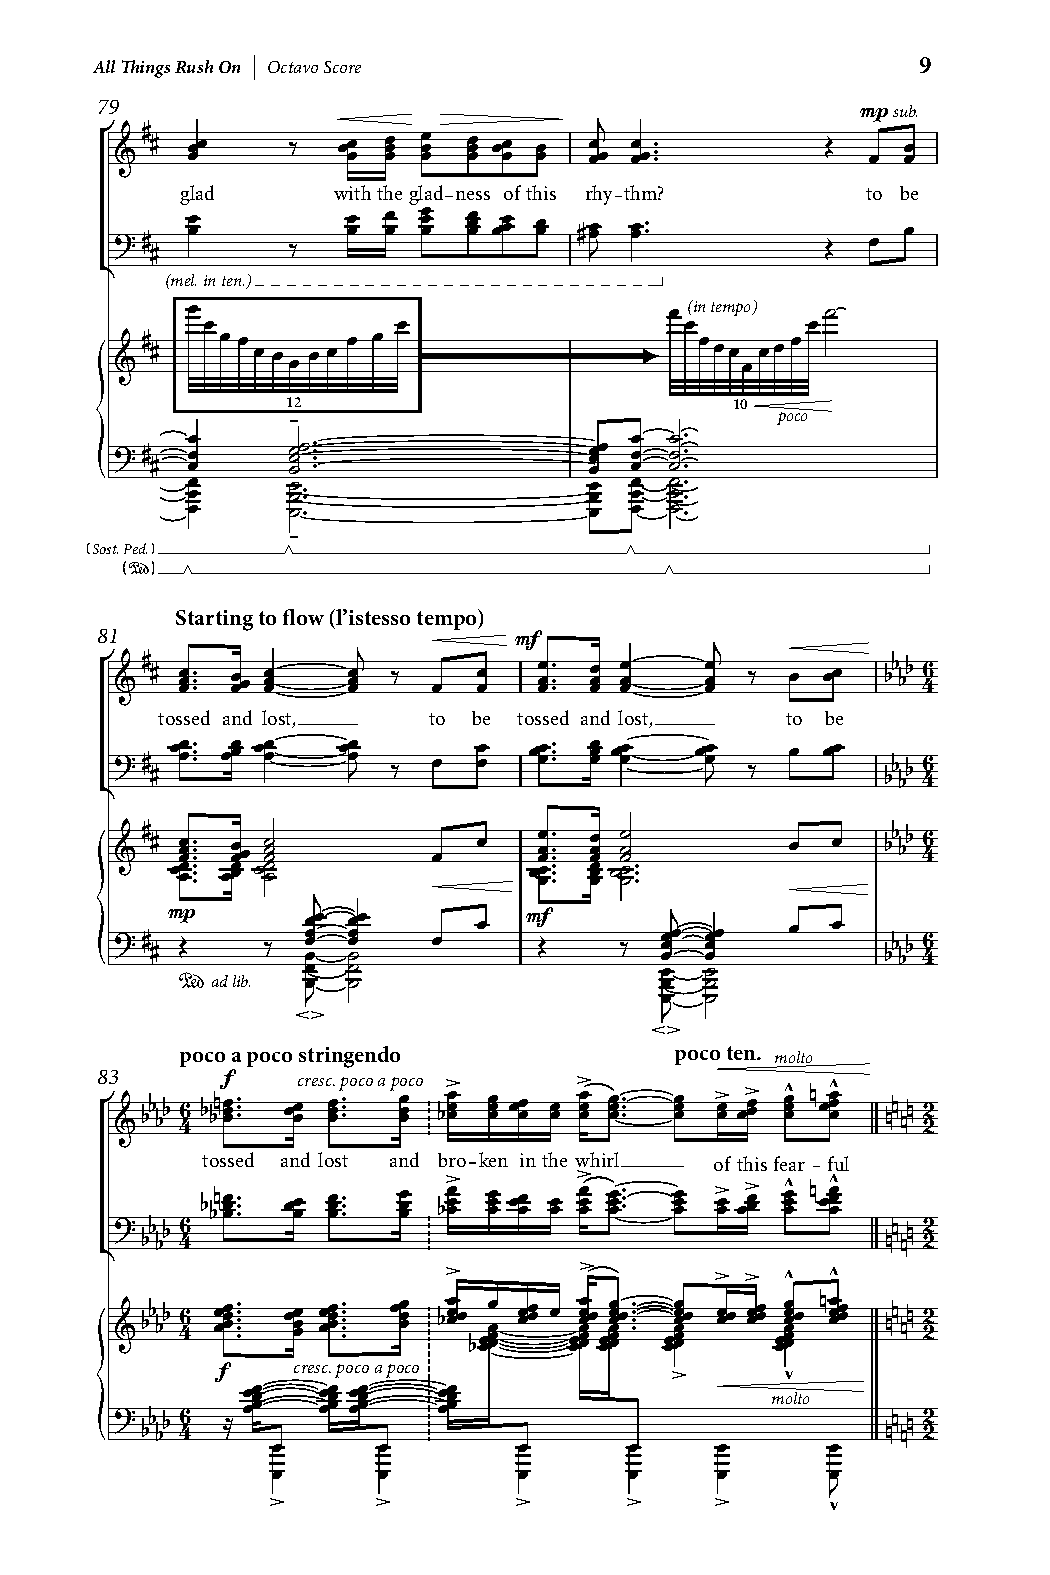
\includegraphics[width=\textwidth]{AllThingsRushOn_pg13.pdf}

	{\scriptsize © 2019 Kieren MacMillan $\bullet$
		\emph{The excerpt is reproduced with the kind permission of the publisher.}}
}

  \headerbox{Contemporary Music}{name=keller,column=4,span=1,aligned=rushon}{
	Excerpt from Hermann Keller's composition for speaking cellist\\
	“Ihr sollt die Wahrheit erben”

    %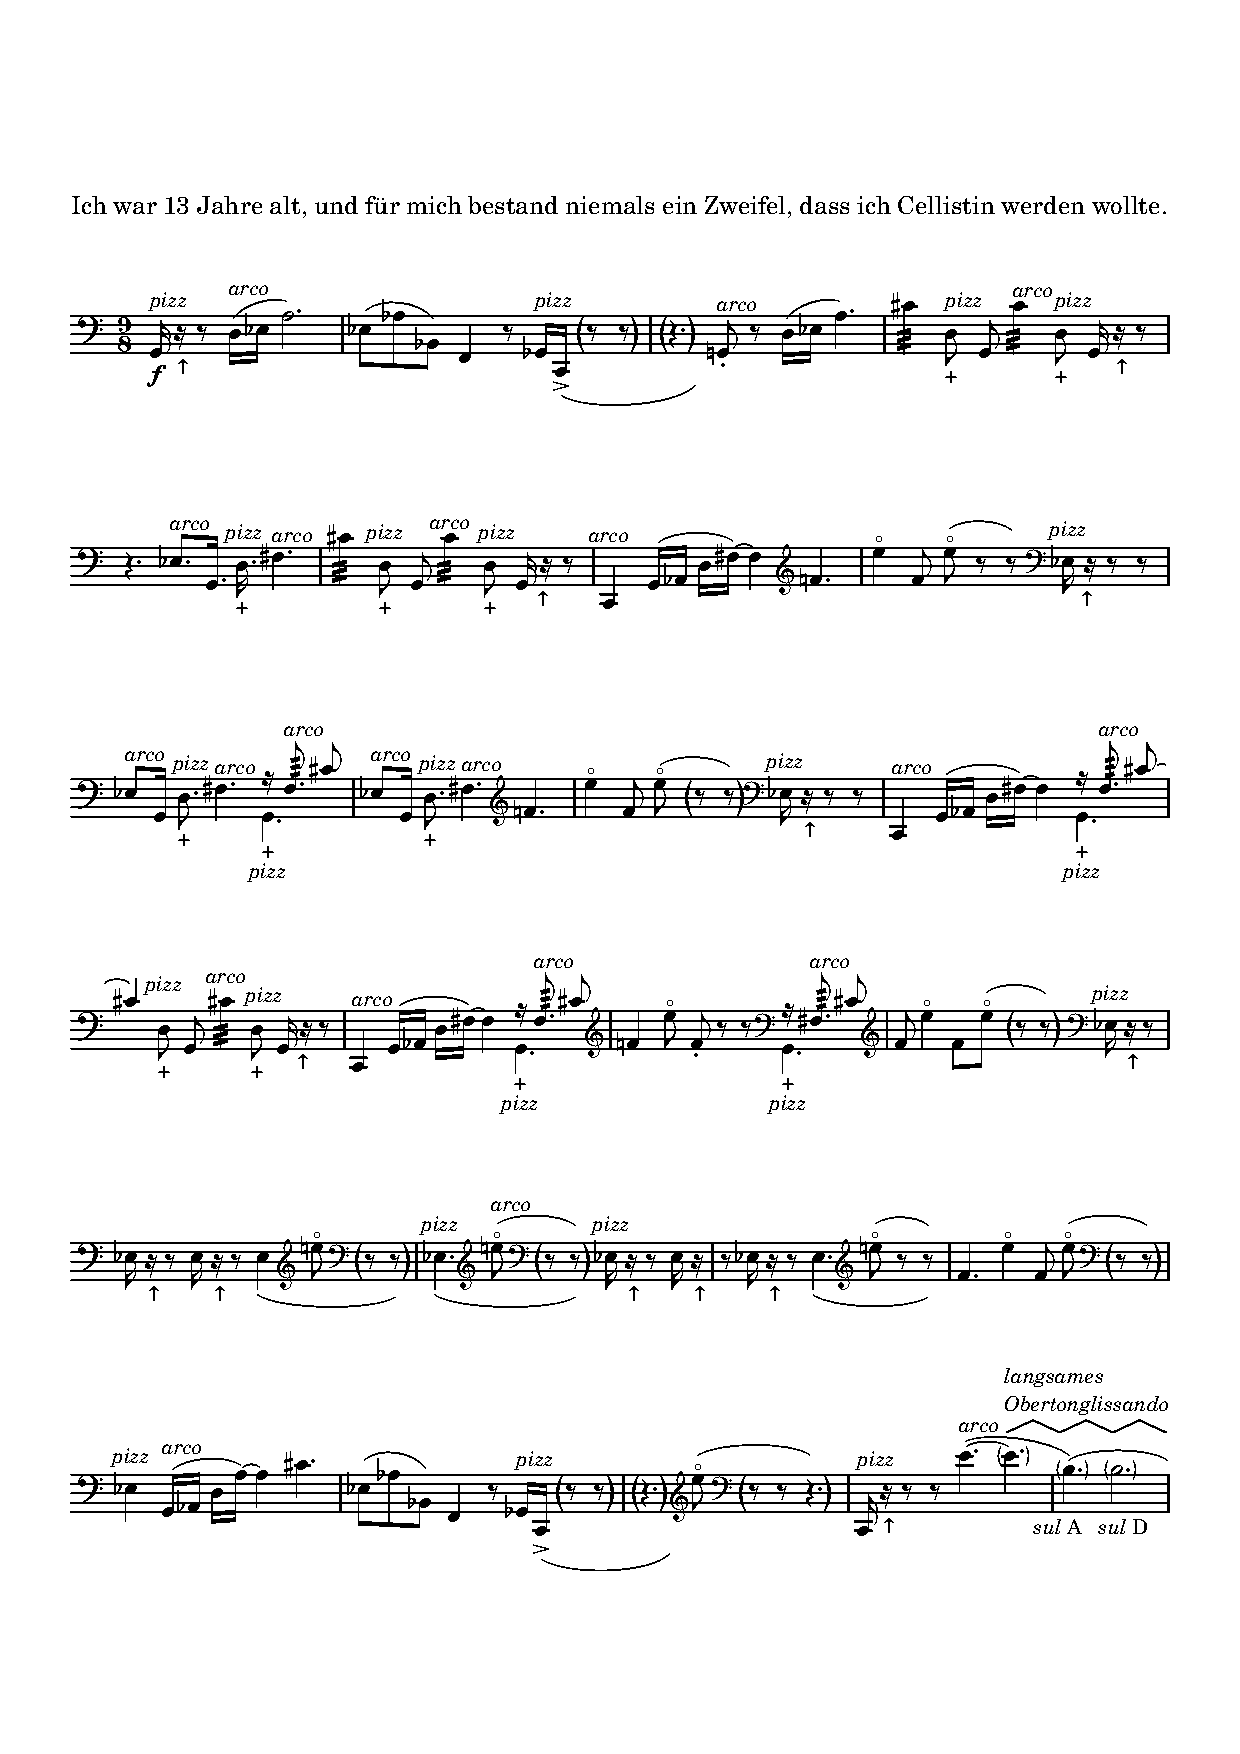
\includegraphics[width=.5\textwidth]{keller-wahrheit1}
    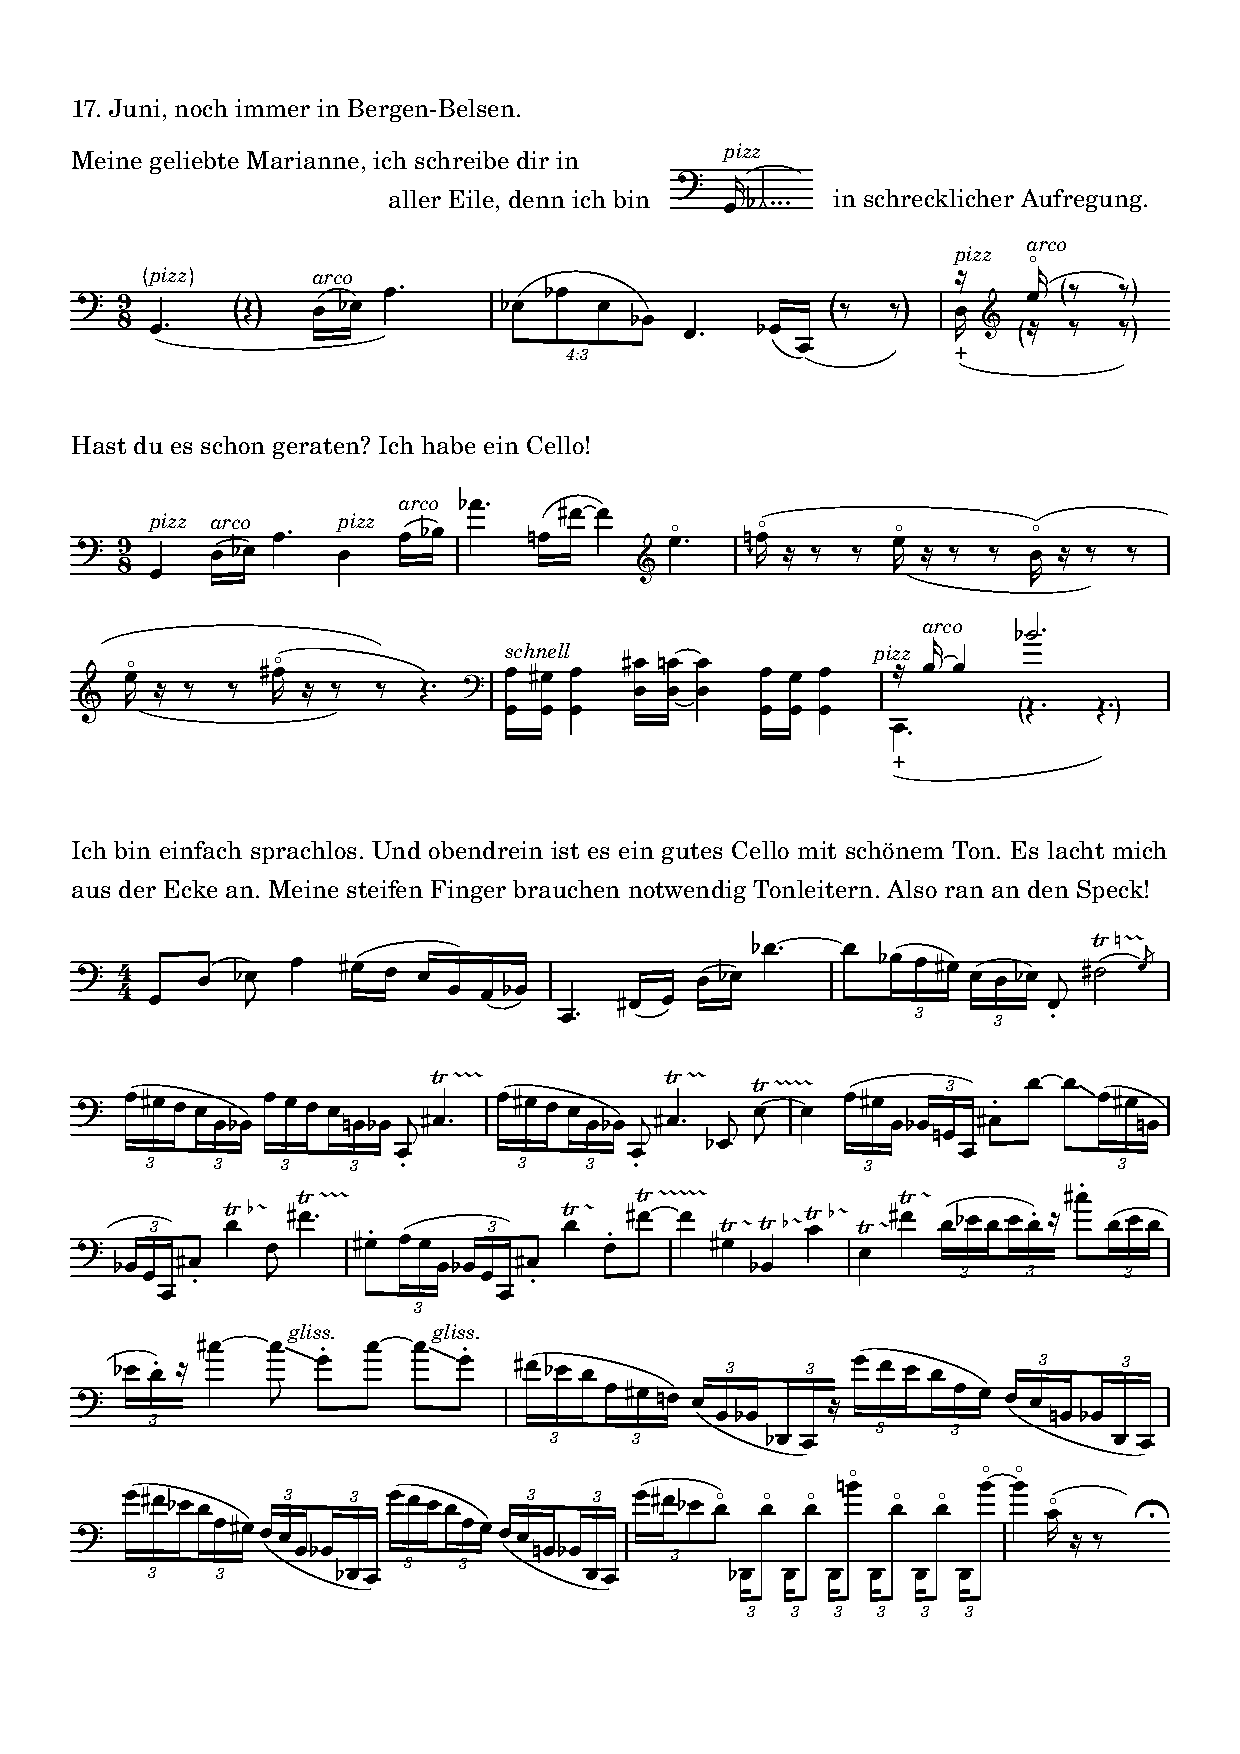
\includegraphics[width=\textwidth]{keller-wahrheit2}

	{\scriptsize © 2019 Edition Juliane Klein, Berlin $\bullet$
	\emph{The excerpt is reproduced with the kind permission of the publisher.}}
    }
  \headerbox{}{column=0,span=5,row=.875}{
  	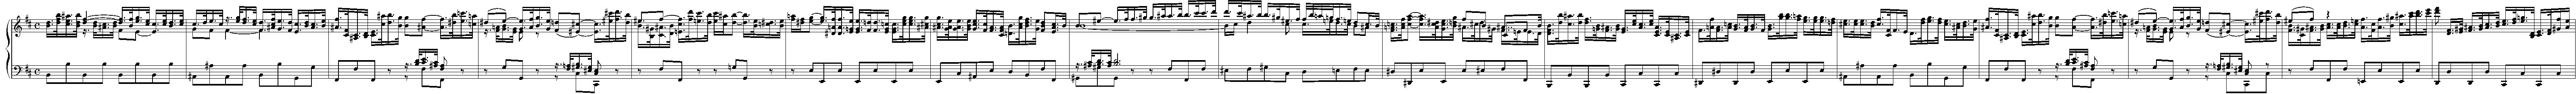
\includegraphics[width=\textwidth]{salzburg-poster.pdf}
  	
  	\hfill \small Poster created by Jan-Peter Voigt, Erlend Aasland, Urs Liska
  }

\end{poster}
\end{document}
